\subsection{El problema}

	La gran cantidad de imágenes y documentos existentes en la actualidad ha motivado el desarrollo de modelos y métodos robustos para la búsqueda automatizada de información con el objeto de reducir los problemas asociados a su análisis e interpretación. La extracción y reconocimiento de texto en imágenes naturales, es decir, imágenes de escenas de la vida diaria y/o adquiridas en condiciones no controladas, es un problema de gran interés tanto desde el punto de vista teórico como del de las aplicaciones.  Sin embargo, a diferencia del problema de reconocimiento de texto en documentos escaneados, el reconocimiento de texto en imágenes naturales plantea problemas difíciles de abordar mediante el uso de técnicas tradicionales basadas en OCR (\textit{Optical Character Recognition}, por su denominación en inglés). Esto resulta evidente si se consideran los cambios en la iluminación, los distintos puntos de vista, las diferentes tipografías, estilos, etc. que se ven reflejadas en imágenes de la vida cotidiana.
	
			\begin{figure}[htbp]
				\centering
				\centerline{
					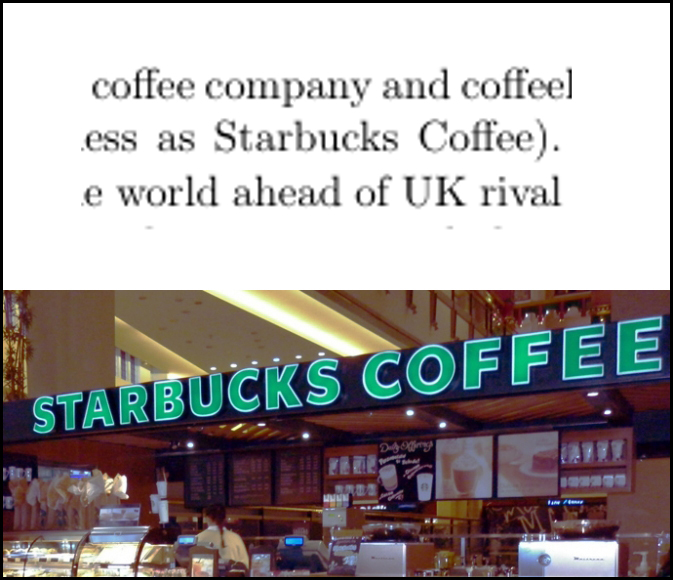
\includegraphics[scale=0.31]{img/ocr_vs_naturalImg_3.jpg}
				}
				\caption[OCRvsNaturales]{La parte superior muestra la imagen de un texto representada con una fuente de computadora donde se puede observar las palabras ``Starbucks Coffee''. La parte inferior expone las mismas palabras pero en una escena natural. Esto se realiza con el objetivo de observar las diferencias que hay entre analizar texto simple (fuente de computadora) y realizar el mismo trabajo en una imagen real}
				\label{fig: Optophone}
			\end{figure}
			
	En la literatura, uno de los esquemas de procesamiento más utilizados ha sido la detección de regiones dentro la imagen que corresponden a texto, su rectificación y la posterior aplicación de técnicas estándar de OCR (Kumar et al., 2007). Sin embargo, esta clase de técnicas se encuentra limitada a los escenarios en donde el OCR funciona correctamente, p.ej. en el reconocimiento de texto impreso (De Campos et al., 2009).

	Recientemente, se propuso un modelo (Wang et al., 2011) que emplea un esquema basado en técnicas de reconocimiento conocidas de la literatura de \textit{reconocimiento de objetos} (Navneet Dalal et al., 2005). En este caso, cada carácter alfanumérico se considera como un objeto a detectar y, empleando un conjunto de muestras de entrenamiento, se genera un modelo de clasificación mediante técnicas de aprendizaje supervisado (Christopher M. Bishop, 2007). Dada una nueva imagen, cada uno de estos clasificadores genera un conjunto de hipótesis sobre la presencia (y su ubicación) de cada símbolo alfanumérico en particular. Estas detecciones se utilizan luego en la detección de palabras específicas a partir de un léxico predefinido. Una particularidad del modelo propuesto por Wang et. al es la utilización de imágenes \textit{sintéticas} (generadas mediante simulación) en la generación de muestras de entrenamiento. Este enfoque reduce el problema de tener que recolectar una gran cantidad de imágenes naturales lo cual consume tiempo y esfuerzo. Mediante diferentes tipos de transformaciones, se busca crear un conjunto de imágenes de caracteres lo más parecido posible a uno real.
	